%%%%%%%%%%%%%%%%%%%%%%%%%%%%%%%%%%%%%%%%%%%%%%%%%%%%%%%%%%
% # Adult L1 Research on Resumption vs. Gapping in Relative Clauses
%%%%%%%%%%%%%%%%%%%%%%%%%%%%%%%%%%%%%%%%%%%%%%%%%%%%%%%%%%

\addtocontents{toc}{\protect\newpage}

\chapter{Adult L1 Research on Resumption vs. Gapping in Relative Clauses}\label{ch-resumption}

% \excnt=84

This chapter reviews the adult L1 experimental literature on the acceptability and processing of resumptive vs. gapped RCs, and, where appropriate, of resumptive vs. gapped \textit{wh}-questions as another type of A-bar dependency. Although the discussion is mostly limited to studies involving L1-English adults, I also go over a few studies testing L1-Hebrew adults to illustrate that experimental findings tend to show that processing effects for resumption hold similarly for intrusive resumption languages and grammatical resumption languages (\cite{meltzer-asscher2021}, p.~179).\footnotemark{} The chapter is organized as follows: I begin in Section~\ref{res-wellformedness} by exploring how mainstream views on the well-formedness of English resumptive RCs have evolved over the years. In Sections~\ref{res-comprehension}--\ref{res-morgan}, I turn to the effect that resumption has on real-time language production and comprehension, reviewing arguments for (and in the case of comprehension, also against) the idea that resumption reduces strain on the processor. In Section~\ref{res-gapping}, I go on to present a more nuanced approach to conceptualizing the effect that resumption has in real-time sentence processing---one in which gapping and resumption alike have the capacity to either facilitate or hinder processing under different conditions. Section~\ref{res-conclusion} concludes the chapter.

\footnotetext{For the sake of consistency and ease of comparison, I have relabeled some factors in the studies reviewed below.}

%========================================================%
\section{Resumption and well-formedness}\label{res-wellformedness}
%========================================================%

As we saw in Section \ref{pro-distribution}, languages differ with regard to the environments where resumption is permitted to occur. In the case of English, there is widespread agreement that resumption is not allowed in short-distance RCs. Consider, for instance, the short-distance RCs in (\ref{ex-english-resump}), which are ill-formed with a resumptive pronoun (RP) but would have been well-formed if a gap had been used instead.

\pex\label{ex-english-resump} 
\a \ljudge*the man [that \boxing{he} hired Tina] ~ (SU)
\a \ljudge*the man [that Tina hired \boxing{him}] ~ (DO)
\a \ljudge*the man [that Tina gave the money to \boxing{him}] ~ (IO)
\a \ljudge*the man [that Tina talked about \boxing{him}] ~ (OBL)
\a \ljudge*the man [that Tina met \boxing{his} mother] ~ (GEN)
\a \ljudge*the man [that Tina is taller than \boxing{him}] ~ (OCOMP)
\xe 

\noindent The issue of whether English permits resumption in certain types of long-distance RCs is more controversial. \textcite{ross1967}, for instance, claimed that resumption can repair island constraint violations to the point that the resulting RCs are ``perfectly natural'' (p.~432), at least in some registers of spoken English (see~also \cite{kayne1981}, p.~115). An example sentence from Ross's dissertation displaying a resumptive RC that extends into a complex NP island is provided in~(\ref{ex-ross}).

\begin{samepage}
\ex\label{ex-ross}I just saw that girl [who Long John's claim [that \boxing{she} was a Venusian] made all the headlines].\par\nobreak\vspace{5pt}
\hfill (adapted from \cite{ross1967}, p. 432, (6.154a))
\xe 
\end{samepage}

\noindent Resumption has traditionally been viewed as a `last resort' strategy for relativization in English; that is to say, resumptive RCs can be well-formed, but only when the gapped version of the RC would violate an island constraint (\cite{chomsky1995}; \cite{ross1967}; \cite{shlonsky1992}). In this sense, resumption has been thought of as `amnestying' island violations in English (\cite{kroch1981}, p.~125; see~also \cite{erteschik-shir1992}, p.~90).

However, experimental research carried out over the past few decades  (\cite{alexopoulou.keller2007}; \cite{beltrama.xiang2016}; \cite{han.etal2012}; \cite{heestand.etal2011}; \cite{keffala2011}; \cite{keffala.goodall2011}; \cite{mcdaniel.cowart1999}; \cite{omaki.nakao2010}; \cite{polinsky.etal2013}) has consistently shown that L1-English speakers assign low acceptability ratings to resumptive RCs and resumptive \textit{wh}-questions both in nonislands and in islands, which casts doubt on the idea that resumption is ever grammatical in English.

Alexopoulou and Keller's (\citeyear{alexopoulou.keller2007}) study testing whether resumption can rescue English island violations in \textit{wh}-questions is one of the most frequently cited works in this line of research. Their experiments consisted of acceptability judgment tasks (AJTs) administered to adult native speakers of English, German, and Greek. The design of the English AJT is summarized in Table~\ref{tblr:alexopoulou}.

\begin{longtblr}[caption={\textcite{alexopoulou.keller2007}: English acceptability judgment task}, label={tblr:alexopoulou}]{colspec={|X|}, rowhead=0, rows={font=\raggedright\setstretch{1}}}\hline
\textbf{Participants:} 55 L1-English adults \vspace{5pt}\rule{0pt}{10pt}\\*
\textbf{Factors:} 4 × 2 × 2 design crossing \textsc{island} (nonisland without complementizer vs. nonisland with complementizer vs. \textit{whether}-island vs. RC island), \textsc{embedding} (single vs. double), and \textsc{dependency} (gap vs. RP) \vspace{5pt}\\*
\textbf{Stimuli:} 162 items (9 lexicalizations each of 16 main critical conditions and 2 control conditions) divided among 9 running lists; each participant rated 1 item per condition and 18 fillers; all \textit{wh}-questions in the stimuli targeted the direct object position \vspace{5pt}\\
\textbf{Procedure:} Participants read sentences and rated them using magnitude estimation (\cite{bard.etal1996}).\vspace{5pt}\\
\textbf{Conditions (p. 117, (11)--(13)):} \vspace{5pt}\\*
\begin{varwidth}{\linewidth}\begin{enumerate}[\bfseries (a),itemsep=5pt] 
\item \textbf{Control sentences:}\par\nobreak
Who will we fire \{\_\_/*him\}?
\item \textbf{Singly embedded nonisland without complementizer:}\par\nobreak
Who does Mary claim we will fire \{\_\_/*him\}?
\item \textbf{Doubly embedded nonisland without complementizer:}\par\nobreak
Who does Jane think Mary claims we will fire \{\_\_/*him\}?
\item \textbf{Singly embedded nonisland with complementizer:}\par\nobreak
Who does Mary claim that we will fire \{\_\_/*him\}?
\item \textbf{Doubly embedded  nonisland with complementizer:}\par\nobreak
Who does Jane think that Mary claims that we will fire \{\_\_/*him\}?
\item \textbf{Singly embedded \textit{whether}-island:}\par\nobreak
Who does Mary wonder whether we will fire \{*\_\_/*him\}?
\item \textbf{Doubly embedded \textit{whether}-island:}\par\nobreak
Who does Jane think that Mary wonders whether we will fire \{*\_\_/*him\}?
\item \textbf{Singly embedded RC island:}\par\nobreak
Who does Mary meet the people that will fire \{*\_\_/*him\}?
\item \textbf{Doubly embedded RC island:}\par\nobreak
Who does Jane think that Mary meets the people that will fire \{*\_\_/*him\}?
\end{enumerate}\end{varwidth}\vspace{5pt}\\\hline
\end{longtblr}

The mean ratings for gap trials were very high for control sentences and above the zero mark on the logit scale in all the nonisland conditions, suggesting that most participants found them to be acceptable. By contrast, the mean ratings for gap trials were lower in all the island conditions, particularly in the RC island conditions, where they were roughly on par with RP trials. Importantly, the ratings for RP trials were low across the board, suggesting that most participants considered them to be unacceptable. Although RP trials in nonisland conditions became slightly more acceptable at deeper levels of embedding, the means remained on the lower half of the logit scale and never overtook the mean ratings for gap trials. Alexopoulou and Keller took these results as evidence (a) that resumption is ungrammatical in English and (b) that it cannot rescue island violations. However, they themselves acknowledged that resumption is only rarely observed in \textit{wh}-questions, so the unacceptability of RPs in this context does not necessarily preclude their acceptability in other types of A-bar dependencies, such as RCs, where they are much more likely to be found in spontaneous production data (p.~149ff).

Following up on Alexopoulou and Keller's study, \textcite{heestand.etal2011} administered a series of AJTs to L1-English adults to test the acceptability of resumption vs. gapping in both RCs and \textit{wh}-questions. Each experiment had a 2~×~3 design crossing \textsc{construction} (RC vs. \textit{wh}-question) and \textsc{dependency} (gap in nonisland vs. gap in island vs. RP in island), as shown in Table~\ref{tblr:heestand}.

\begin{longtblr}[caption={\textcite{heestand.etal2011}: Acceptability judgment tasks}, label={tblr:heestand}]{colspec={|X|}, rowhead=0, rows={font=\raggedright\setstretch{1}}}\hline
\textbf{Tasks:} Experiment~1a was an offline AJT examining complex NP islands; Experiment~1b was an offline AJT examining RC islands; Experiment 2 was an online AJT examining RC islands; and Experiment 3 was an online AJT examining adjunct islands \vspace{5pt}\rule{0pt}{10pt}\\*
\textbf{Participants:} 18 in Experiment~1a; 18 in Experiment~1b; 24 in Experiment~2; 24 in Experiment~3; all were L1-English adults \vspace{5pt}\\
\textbf{Factors:} Each experiment had a 2 × 3 design crossing \textsc{construction} (RC vs. \textit{wh}-question) and \textsc{dependency} (gap in nonisland vs. gap in island vs. RP in island) \vspace{5pt}\\
\textbf{Stimuli:} 30 critical items per task (6 conditions × 5 tokens, Latin-squared) and 108 fillers; all RCs and \textit{wh}-questions in the critical stimuli targeted the direct object position \vspace{5pt}\\
\textbf{Procedure:} Participants read sentences and rated them on a 7-point scale ranging from 1~(unacceptable) to 7~(perfectly acceptable). \vspace{5pt}\\
\textbf{Conditions in Experiment 1a -- complex NP islands (p. 141, (4)):} \vspace{5pt}\\*
\begin{varwidth}{\linewidth}\begin{enumerate}[\bfseries (a),itemsep=5pt] 
\item \textbf{RC with island gap/RP:}\par\nobreak
This is the man that the news that the police arrested \{*\_\_/*him\} shocked the public.
\item \textbf{RC with nonisland gap (grammatical control):}\par\nobreak
This is the man that Mary thought that the police arrested \_\_ to protect the president.
\item \textbf{\textit{Wh}-question with island gap/RP:}\par\nobreak
Which man did the news that the police arrested \{*\_\_/*him\} shock the public? 
\item \textbf{\textit{Wh}-question with nonisland gap (grammatical control):}\par\nobreak
Which man did Mary think that the police arrested \_\_ to protect the president? 
\end{enumerate}\end{varwidth}\vspace{5pt}\\
\textbf{Conditions in Experiments 1b and 2 -- RC islands (p. 143, (5)):} \vspace{5pt}\\*
\begin{varwidth}{\linewidth}\begin{enumerate}[\bfseries (a),itemsep=5pt] 
\item \textbf{RC with island gap/RP:}\par\nobreak
This is the man that the policeman who arrested \{*\_\_/*him\} saved the president's life.
\item \textbf{RC with nonisland gap (grammatical control):}\par\nobreak
This is the man that the policeman who arrested the thief saved \_\_.
\item \textbf{\textit{Wh}-question with island gap/RP:}\par\nobreak
Which person did Mary think that the policemen who arrested \{*\_\_/*him\} saved the president's life? 
\item \textbf{\textit{Wh}-question with nonisland gap (grammatical control):}\par\nobreak
Which man did Mary think that the policeman who arrested the thief saved \_\_? 
\end{enumerate}\end{varwidth}\vspace{5pt}\\
\textbf{Conditions in Experiment 3 -- adjunct islands (p. 147, (6)):} \vspace{5pt}\\*
\begin{varwidth}{\linewidth}\begin{enumerate}[\bfseries (a),itemsep=5pt] 
\item \textbf{RC with island gap/RP:}\par\nobreak
This is the dish that, although the chef overcooked \{*\_\_/*it\}, the guests were not upset.
\item \textbf{RC with nonisland gap (grammatical control):}\par\nobreak
This is the dish that, although the chef overcooked the sauce, the guests enjoyed \_\_.
\item \textbf{\textit{Wh}-question with island gap/RP:}\par\nobreak
Which dish did Gina think that, although the chef overcooked \{*\_\_/*it\}, the guests were not upset? 
\item \textbf{\textit{Wh}-question with nonisland gap (grammatical control):}\par\nobreak
Which dish did Gina think that, although the chef overcooked the sauce, the guests enjoyed~\_\_? 
\end{enumerate}\end{varwidth}\\\hline
\end{longtblr}

Gap trials and RP trials both received consistently low ratings in islands, the one exception being in the experiment testing adjunct islands, where gap trials and RP trials were both rated only slightly lower than the grammatical control sentences. Heestand et al. accounted for this unexpected finding by claiming that adjuncts used in the experiment (\textit{although}-adjuncts and \textit{while}-adjuncts) are relatively weak islands that (for reasons yet to be fully understood) cause less severe island effects than other types of islands (p. 149). Overall, these results indicate once again that resumption cannot rescue island violations and that sentences with resumption inside islands tend to receive very low ratings. 

One limitation of the \textcite{heestand.etal2011} study is that the foot of the dependency was always in the direct object position, despite the fact that in English RCs, resumptive nominals tend to be observed more often in subject position than in direct object position (e.g.,~\cite{morgan.wagers2018}). In my own informally-collected corpus (\url{https://osf.io/xwgfz}), resumptive SRCs outnumber resumptive ORCs by a fairly wide margin in the oral production data from individuals I judged to be L1-English speakers (based on, e.g., information I was able to collect on each speaker from a simple internet search---most of the data points were RCs produced by public figures during radio broadcasts).\footnotemark{} 

\footnotetext{Of the 174 relevant tokens, 75 (43\%) are SRCs whereas only 55 (32\%) are ORCs. The remaining 44 tokens are a combination of genitive RCs (22/74 = 13\%), oblique RCs (21/74 = 12\%), and indirect object RCs (1/74 = 1\%).}

\textcite{mcdaniel.cowart1999} was the first study I could find that experimentally tested for a subject-object asymmetry in the acceptability of English resumptive RCs. The AJT they used in their study had a 2~×~2 design crossing \textsc{structure} (SRC vs. ORC) and \textsc{dependency} (gap vs. RP), as shown in Table~\ref{tblr:mcdaniel}.

\begin{longtblr}[caption={\textcite{mcdaniel.cowart1999}: Acceptability judgment task}, label={tblr:mcdaniel}]{colspec={|X|}, rowhead=0, rows={font=\raggedright\setstretch{1}}}\hline
\textbf{Participants:} 36 L1-English adults \vspace{5pt}\rule{0pt}{10pt}\\*
\textbf{Factors:} 2~×~2 design crossing \textsc{structure} (SRC vs. ORC) and \textsc{dependency} (gap vs. RP) \vspace{5pt}\\
\textbf{Stimuli:} 24 critical items (4 conditions × 6 tokens, Latin-squared) and 48 fillers spanning 3~levels of acceptability (acceptable, degraded, and unacceptable); all critical conditions had RC dependencies extending into \textit{wh}-islands \vspace{5pt}\\
\textbf{Procedure:} Participants read sentences and rated them on a 10-point scale ranging from 0~(lowest) to 9~(highest) with a reference sentence at the midpoint. \vspace{5pt}\\
\textbf{Conditions (pp. B16--B18, (2) and (4)):} \vspace{5pt}\\*
\begin{varwidth}{\linewidth}\begin{enumerate}[\bfseries (a),itemsep=5pt] 
\item \textbf{SRC with gap/RP \textit{wh}-island:}\par\nobreak
That's the girl that I wonder when \{*\_\_/*she\} met you.
\item \textbf{ORC with gap/RP in \textit{wh}-island:}\par\nobreak
That's the girl that I wonder when you met \{*\_\_/*her\}.
\end{enumerate}\end{varwidth}\\\hline
\end{longtblr}

Ratings were low across all four critical conditions, and RP trials were rated significantly higher than gap trials only in SRCs. This difference was not due to an ameliorating effect of resumption, however: RP trials were rated more or less the same across both levels of \textsc{dependency}. Instead, the difference stemmed from the fact that the subject gap condition was rated significantly lower than the other three conditions, perhaps---McDaniel and Cowart suggest (p.~B18)---because it violates an additional constraint on English grammar such as the Empty Category Principle (\cite{chomsky1981}). Later studies by \textcite{keffala.goodall2011} and \textcite{han.etal2012} have found the same general pattern of results for adjunct islands, complex NP islands, and RC islands. 

An increasing number of researchers have started to treat English resumption as an ungrammatical repair device (\cite{alexopoulou.keller2007}, p.~150; \cite{chacon2015}, p.~89; \cite{kroch1981}, p.~131ff; \cite{sells1984}, p.~461), calling it `intrusive' resumption (\cite{sells1984}, p.~27) or `processing' resumption (\cite{asudeh2004}, p.~295) to distinguish it from the grammatical resumption observed in languages such as Hebrew. Even if resumptive RCs are ill-formed, though, it is undeniable that they do occur in the spontaneous speech of L1-English adults (\cite{asudeh2004}; \cite{cann.etal2005}; \cite{prince1990}). Example (\ref{ex-ferreira-swets}), from a public radio broadcast, is a resumptive RC that extends into a \textit{wh}-island. By some estimates, we can expect to hear such sentences about once or twice in the average day (\cite{ferreira.swets2005}, p.~263).

\ex\label{ex-ferreira-swets}
We're afraid of things [that we don't know [what \boxing{they} are]].\par\nobreak\vspace{5pt}
\hfill (adapted from \cite{ferreira.swets2005}, p. 263)
\xe 

\noindent It has been suggested that such utterance types are produced not because they are acceptable but instead because they facilitate processing. \textcite{kroch1981}, for instance, argued that English resumption is a processing artifact (see~p.~131ff)---the natural result of a processor that has limited planning capacity and therefore occasionally begins to construct an RC without realizing that it will need to extend the dependency into a domain where gapping is prohibited. Inserting a resumptive element in such cases gives the speaker a means of reestablishing coreference and continuing the production chain without needing to stop and reformulate. The result is something that is ill-formed but at least easier to process than the corresponding RC with an illicit gap (for~similar accounts, see \cite{asudeh2004}, p.~297ff; \cite{chacon2015}, p.~150ff; \cite{chacon2019}, p.~3).

Although the standard assumption among linguists these days is that resumption is ungrammatical in languages like English, it bears mentioning that some researchers persist in treating resumption as a fundamentally grammatical option for English relativization, at least in certain syntactic domains and in certain communicative contexts (see~\cite{creswell2002}; \cite{goodall2017}; \cite{radford2019}). \textcite{goodall2017}, for instance, holds that English resumption in islands is a grammatical option on par with gapping in non-islands, with the low acceptability of resumptive RCs and resumptive \textit{wh}-questions resulting from the processing costs required for shifting from a gapped dependency to a resumptive dependency:

\begin{samepage}\begin{quote}
Unlike gaps, pronouns do not unambiguously resolve the \textit{wh}-dependency, so when the processor encounters resumptive pronouns, one would expect it to proceed normally (i.e.,~attempt to locate an entity in the recent discourse to which the pronoun could refer), while leaving the \textit{wh}-dependency open. Once it is clear that we are outside the scope of the [operator] and that a gap will no longer be possible \dots{}, the processor must then reanalyze the pronoun so that it is interpreted as resumptive.
\par\vspace{5pt}
\hfill (\cite{goodall2017}, p. 71)
\end{quote}\end{samepage}
\vspace{-12pt}

%========================================================%
\section{How resumption might assist with comprehension}\label{res-comprehension}
%========================================================%

Early attempts at explaining how resumption might facilitate processing focused mostly on comprehension. One of these theories, which still has currency today, is that resumptive elements assist with comprehension by explicitly marking the foot of the dependency, thereby making it easier to locate (\cite{beltrama.xiang2016}, p.~17ff; \cite{hawkins1999}, p.~257; \cite{hofmeister.norcliffe2013}, p.~237; \cite{keenan.comrie1977}, p.~92; see~also \cite{meltzer-asscher2021}, p.~179). This is likely to be especially helpful within island configurations, since there is experimental research indicating that the active gap search is suspended inside islands (\cite{omaki.schulz2011}; \cite{phillips2006}; \cite{stowe1986}; \cite{traxler.pickering1996}), as illustrated in (\ref{ex-suspend-search}).

\pex\label{ex-suspend-search}
\a Successful dependency resolution with gap following adjunct island:\par\nobreak
\tikz{
\node (rectA) at (0,0) {\strut \phantom{*}the dish [ that, [};
\node (rectB) [rectangle, draw, thick, base right=0pt of rectA] {\strut although the chef overcooked the sauce};
\node (rectC) [base right=0pt of rectB] {\strut ], the guests enjoyed \_\_ ]};
\node(textA) [rectangle, fill=white] at ([yshift=0pt]rectB.south) {\small\sc adjunct island};
\draw[|-|, thick] ([yshift=21pt,xshift=18pt]rectA.center) -- ([yshift=21pt,xshift=38pt]rectC.center) node[midway,rectangle,fill=white]{Filler storage};
\draw[<-, thick] ([yshift=4pt,xshift=47pt]rectC.south) -- +(0, -0.6) -| ([yshift=4pt,xshift=-8pt]rectA.south) node[pos=0.25,rectangle,fill=white]{Filler integration};
}\label{ex-suspend-search-a}
\a Unsuccessful dependency resolution with gap inside adjunct island:\par\nobreak
\tikz{
\node (rectA) at (0,0) {\strut *the dish [ that, [};
\node (rectB) [rectangle, draw, thick, base right=0pt of rectA] {\strut although the chef overcooked \_\_};
\node (rectC) [base right=0pt of rectB] {\strut ], the guests were not upset ]};
\node(textA) [rectangle, fill=white] at ([yshift=0pt]rectB.south) {\small\sc adjunct island};
\draw[|-|, thick] ([yshift=21pt,xshift=18pt]rectA.center) -- ([yshift=21pt]rectC.east) node[midway,rectangle,fill=white]{Filler storage};
\draw[Rays-, thick] ([yshift=4pt]rectC.south east) -- +(0, -0.6) -| ([yshift=4pt,xshift=-8pt]rectA.south) node[pos=0.25,rectangle,fill=white]{Abandonment of dependency};
}\label{ex-suspend-search-b}
\a Successful dependency resolution with RP inside adjunct island:\par\nobreak
\tikz{
\node (rectA) at (0,0) {\strut *the dish [ that, [};
\node (rectB) [rectangle, draw, thick, base right=0pt of rectA] {\strut although the chef overcooked it};
\node (rectC) [base right=0pt of rectB] {\strut ], the guests were not upset ]};
\node(textA) [rectangle, fill=white] at ([yshift=0pt]rectB.south) {\small\sc adjunct island};
\draw[|-|, thick] ([yshift=21pt,xshift=18pt]rectA.center) -- ([yshift=21pt,xshift=73pt]rectB.center) node[midway,rectangle,fill=white]{Filler storage};
\draw[->, thick] ([yshift=5pt,xshift=73pt]rectB.south) -- +(0, -0.6) -| ([yshift=5pt,xshift=-8pt]rectA.south) node[pos=0.25,rectangle,fill=white]{Antecedent identification};
}\par\nobreak\label{ex-suspend-search-c}
\hfill (based on stimuli from \cite{heestand.etal2011}, p. 147, (6))
\xe 

\noindent In (\ref{ex-suspend-search-b}), the parser cannot integrate the filler inside the adjunct island, which leads to eventual abandonment of the dependency. In (\ref{ex-suspend-search-c}), on the other hand, the RP inside the island clause triggers a search for a viable antecedent (\cite{alexopoulou.keller2007}, p.~144; \cite{erteschik-shir1992}, p.~91; \cite{hofmeister.norcliffe2013}, p.~238), which in this case results in accurate (albeit ungrammatical) dependency resolution. Such resumption arguably allows the dependency to be resolved even when the gap search has been suspended (\cite{meltzer-asscher2021}, p.~180). 

Many resumptive elements also carry overt marking for features such as animacy, person, number, and gender that can facilitate the establishment of a coreferential relationship with the head noun (\cite{beltrama.xiang2016}, p.~18; \cite{hofmeister.norcliffe2013}, p.~227; \cite{meltzer-asscher2021}, p.~179). In (\ref{ex-antecedent-search}), for instance, the RP \textit{him} is marked for the features third person, singular, and masculine which together single out the head noun \textit{man} as the only possible antecedent within the bounds of the sentence.

\ex\label{ex-antecedent-search}Antecedent search in a resumptive RC:\par\nobreak
\begin{tikzpicture}
\node (rectA) [rectangle, draw, thick] at (0,-1) {\strut Mary};
\node (dotA) [base right=0pt of rectA] {\strut knows};
\node (rectB) [rectangle, draw, thick, base right=0pt of dotA] {\strut the man};
\node (dotB) [base right=0pt of rectB] {\strut [ that};
\node (rectC) [rectangle, draw, thick, base right=0pt of dotB] {\strut I};
\node (dotC) [base right=0pt of rectC] {\strut wonder [};
\node (rectD) [rectangle, draw, thick, base right=0pt of dotC] {\strut which detectives};
\node (dotD) [base right=0pt of rectD] {\strut arrested};
\node (rectE) [rectangle, draw, thick, fill=gray!15, base right=0pt of dotD] {\strut him};
\node (rectF) [base right=0pt of rectE] {\strut ] ].};
\node(textA) [above=18pt of rectA.base, anchor=base] {{\sy ✗}};
\node(textB) [above=18pt of rectB.base, anchor=base] {{\sy ✓}};
\node(textC) [above=18pt of rectC.base, anchor=base] {{\sy ✗}};
\node(textD) [above=18pt of rectD.base, anchor=base] {{\sy ✗}};
\node(featA) [below=20pt of rectA.base, anchor=base] {{\small\sc [3fs]}};
\node(featB) [below=20pt of rectB.base, anchor=base]{{\small\sc [3ms]}};
\node(featC) [below=20pt of rectC.base, anchor=base] {{\small\sc [1s]}};
\node(featD) [below=20pt of rectD.base, anchor=base] {{\small\sc [3p]}};
\node(featE) [below=20pt of rectE.base, anchor=base]{{\small\sc [3ms]}};
\draw[->, thick] (featE.south) -- +(0, -0.3) -| (featB.south);
\end{tikzpicture}
\xe 

An additional way that resumptive elements may ease comprehension is by giving the processor extra time to resolve the dependency before encountering the remainder of the sentence (\cite{hofmeister.norcliffe2013}, p.~239; \cite{meltzer-asscher2021}, p.~179). Because resumptive nominals do not introduce new discourse referents, the reasoning goes, they give the processor a short reprieve before having to contend with the next word that does introduce a discourse referent. This reprieve, moreover, comes at a critical time in the processing of the sentence: at the precise moment when the RC dependency is being resolved.

%========================================================%
\section{How resumption might assist with production}\label{res-production}
%========================================================%

Asudeh's (\citeyear{asudeh2004,asudeh2011,asudeh2012}) widely cited approach to how resumption facilitates RC production in English begins with the observation that well-formedness is evaluated both at the global level (sentence by sentence) and at the local level (clause by clause). Sentences with an RC whose gap is in a nonisland are both globally well-formed and locally-well formed (with every verb having its required arguments once the filler is integrated at the gap site), as shown in (\ref{ex-asudeh-a}). Sentences with an RC whose gap is in an island, by contrast, are both globally ill-formed (because the filler fails to be integrated before the sentence ends) and locally ill-formed (because the verb in the island is missing one of its arguments), as shown in (\ref{ex-asudeh-b}). Inserting a resumptive nominal may not repair the global ill-formedness of the sentence, but it can at least restore local well-formedness by ensuring that the verb in the island has all the arguments it requires, as shown in (\ref{ex-asudeh-c}); this, in turn, helps speakers maintain coreference when gapped dependencies break down, decreasing the chances that they will have to pause and reformulate.

\pex\label{ex-asudeh}
\a Gap in nonisland:\par\nobreak
\tikz{
\node[rectangle, draw, thick] (rectA) at (0,0) {\strut This is a donkey};
\node (that) [rectangle, base right=5pt of rectA] {\strut [ that};
\node (rectB) [rectangle, draw, thick, minimum size=.6cm, base right=5pt of that] {\strut I think};
\node (where) [rectangle, base right=5pt of rectB] {\strut [};
\node (rectC) [rectangle, draw, thick, minimum size=.6cm, base right=3pt of where] {\strut \_\_ lives in Brazil};
\node (period) [rectangle, base right=5pt of rectC] {\strut ] ].};
\node(textA) at ([yshift=-10pt]rectA.south) {{\sy ✓} Well-formed};
\node(textB) at ([yshift=-10pt]rectB.south) {{\sy ✓} Well-formed};
\node(textC) at ([yshift=-10pt]rectC.south) {{\sy ✓} Well-formed};
\draw[->, thick] ([yshift=-5pt,xshift=20pt]rectA.north) -- ([yshift=10pt,xshift=20pt]rectA.north) -- ([yshift=10pt,xshift=-35pt]rectC.north)node[midway,rectangle,fill=white]{Filler integration} -- ([yshift=-7pt,xshift=-35pt]rectC.north);
\draw[|-|, thick] ([yshift=-40pt]rectA.west) -- ([yshift=-40pt]period.east) node[midway,rectangle,fill=white]{{\sy ✓} Globally well-formed};
}\par\nobreak
\textit{Note}. Filler integrated in the lower clause such that \textit{lives} is provided with a subject.\label{ex-asudeh-a}
\a Gap in \textit{wh}-island:\par\nobreak
\tikz{
\node[rectangle, draw, thick, minimum size=.6cm] (rectA) at (0,0) {\strut This is a donkey};
\node (that) [rectangle, base right=5pt of rectA] {\strut [ that};
\node (rectB) [rectangle, draw, thick, minimum size=.6cm, base right=5pt of that] {\strut I don't know};
\node (where) [rectangle, base right=5pt of rectB] {\strut [ where};
\node (rectC) [rectangle, draw, thick, minimum size=.6cm, base right=5pt of where] {\strut \_\_ lives};
\node (period) [rectangle, base right=5pt of rectC] {\strut ] ].};
\node(textA) at ([yshift=-10pt]rectA.south) {{\sy ✓} Well-formed};
\node(textB) at ([yshift=-10pt]rectB.south) {{\sy ✓} Well-formed};
\node(textC) at ([yshift=-10pt]rectC.south) {* Ill-formed};
\draw[->, thick] ([yshift=-5pt,xshift=20pt]rectA.north) -- ([yshift=10pt,xshift=20pt]rectA.north) -- ([yshift=10pt]period.north east) node[midway,rectangle,fill=white]{Gap search};
\draw[|-|, thick] ([yshift=-40pt]rectA.west) -- ([yshift=-40pt]period.east) node[midway,rectangle,fill=white]{* Globally ill-formed};
}\par\nobreak
\textit{Note}. Filler not integrated in the lower clause such that \textit{lives} lacks a subject.\label{ex-asudeh-b}
\a RP in \textit{wh}-island:\par\nobreak
\tikz{
\node[rectangle, draw, thick, minimum size=.6cm] (rectA) at (0,0) {\strut This is a donkey};
\node (that) [rectangle, base right=5pt of rectA] {\strut [ that};
\node (rectB) [rectangle, draw, thick, minimum size=.6cm, base right=5pt of that] {\strut I don't know};
\node (where) [rectangle, base right=5pt of rectB] {\strut [ where};
\node (rectC) [rectangle, draw, thick, minimum size=.6cm, base right=5pt of where] {\strut it lives};
\node (period) [rectangle, base right=5pt of rectC] {\strut ] ].};
\node(textA) at ([yshift=-10pt]rectA.south) {{\sy ✓} Well-formed};
\node(textB) at ([yshift=-10pt]rectB.south) {{\sy ✓} Well-formed};
\node(textC) at ([yshift=-10pt]rectC.south) {{\sy ✓} Well-formed};
\draw[->, thick] ([yshift=-5pt,xshift=20pt]rectA.north) -- ([yshift=10pt,xshift=20pt]rectA.north) -- ([yshift=10pt]period.north east) node[midway,rectangle,fill=white]{Gap search};
\draw[|-|, thick] ([yshift=-40pt]rectA.west) -- ([yshift=-40pt]period.east) node[midway,rectangle,fill=white]{* Globally ill-formed};
}\par\nobreak
\textit{Note}. Overt pronoun in the lower clause provides \textit{lives} with a subject.\par\nobreak\vspace{5pt}
\hfill (based on \cite{asudeh2004}, p. 315, (8.32))\label{ex-asudeh-c}
\xe 

\noindent Although Asudeh's model is usually cited as a means of explaining how resumption is helpful to speakers, he also suggests that maintaining local well-formedness benefits listeners by making it easier to recover the speaker's intended meaning (p. 317ff; see also \cite{beltrama.xiang2016}, p.~17).

%========================================================%
\section{Experimental evidence suggesting that resumption assists with production}\label{res-evidence-production}
%========================================================%

Whereas the earliest theories of how resumption affects RC processing focused on comprehension, some of the first studies experimentally testing for such processing effects looked instead at production (e.g.,~\cite{ferreira.swets2005}; \cite{zukowski.larsen2004}). The \textcite{ferreira.swets2005} study is one of the most frequently cited works in this area of research. It involved two production tasks and two judgment tasks, as summarized in Table~\ref{tblr:ferreira}.

\begin{longtblr}[caption={\textcite{ferreira.swets2005}: Oral elicitation tasks and acceptability judgment tasks}, label={tblr:ferreira}]{colspec={|X|}, rowhead=0, rows={font=\raggedright\setstretch{1}}}\hline
\textbf{Tasks:} Two oral RC elicitation tasks (one with time pressure, one without time pressure) and two acceptability judgment tasks (one with visual presentation of stimuli, one with auditory presentation of stimuli) \vspace{5pt}\rule{0pt}{10pt}\\*
\textbf{Participants:} 30 L1-English adults per elicitation task; no sample sizes given for the judgment tasks; it is unclear if any participants from the elicitation tasks took part in the judgment tasks \vspace{5pt}\\
\textbf{Stimuli:} Each elicitation task had 24 critical items (12 in the \textit{wh}-island SRC condition and 12 in the nonisland SRC condition) and 24 fillers; the target responses in the elicitation tasks served as the stimuli in the judgment tasks \vspace{5pt}\\
\textbf{Procedure:} In the elicitation tasks, participants saw sets of pictures accompanied by descriptive sentences and answered questions about them (e.g.,~\textit{Which donkey is this?}). In the judgment tasks, participants read or listened to sentences and rated them on a 5-point scale ranging from 1~(perfect) to 5~(awful). \vspace{5pt}\\
\textbf{Target response for each condition in the elicitation tasks (p. 271, (3)):} \vspace{5pt}\\*

\begin{varwidth}{\linewidth}\begin{enumerate}[\bfseries (a),itemsep=5pt] 
\item \textbf{\textit{Wh}-island SRC condition:}\par\nobreak
*This is a donkey that I don't know where \boxing{it} lives.
\item \textbf{Nonisland SRC condition:}\par\nobreak
\phantom{*}This is a donkey that \boxing{\_\_} doesn't know where it lives.
\end{enumerate}\end{varwidth}\\\hline
\end{longtblr}

\noindent Participants produced resumptive RCs at high rates in the \textit{wh}-island SRC condition: 67\% for the task without time pressure and 56\% for the task with time pressure. In the follow-up judgment tasks, participants tended to reject trials with RPs in islands and to accept trials with gaps in nonislands. Ferreira and Swets take these results as evidence that English resumptive RCs are marginal at best in terms of grammaticality but that they are still preferred over gapped RCs when speakers are induced into relativizing from islands.

In another production study, this time in the written mode, \textcite{morgan.wagers2018} elicited ORCs and SRCs in six syntactic environments associated with (what was presumed to be) increasing difficulty of relativization, ranging from the singly embedded nonisland condition (Emb1---easiest) to the adjunct island condition (Adjunct---hardest), as shown in Table~\ref{tblr:morgan-wagers}.

\begin{longtblr}[caption={\textcite{morgan.wagers2018}: Written RC elicitation task}, label={tblr:morgan-wagers}]{colspec={|X|}, rowhead=0, rows={font=\raggedright\setstretch{1}}}\hline
\textbf{Participants:} 42 L1-English adults (after exclusions) \vspace{5pt}\rule{0pt}{10pt}\\*
\textbf{Factors:} 2 × 6 design crossing \textsc{structure} (SRC vs. ORC) and \textsc{embedding domain} (singly embedded nonisland vs. doubly embedded nonisland vs. \textit{wh}-island vs. object-modifying complex NP island vs. subject-modifying complex NP island vs. adjunct island) + 3 control conditions eliciting short-distance SRCs \vspace{5pt}\\
\textbf{Stimuli:} 600 items (15 conditions × 40 lexicalizations); it is unclear how many items were seen by each participant \vspace{5pt}\\
\textbf{Procedure:} Participants were presented with a base sentence (e.g.,~\textit{The ogre claims a prince slayed the troll}) and a prompt (e.g.,~\textit{There's a prince that...}) and responded by writing a continuation to the prompt (e.g.,~\textit{...the ogre claims slayed the troll}). \vspace{5pt}\\
\textbf{Target response for each condition with gapping/resumption (p. 84, Table 1):} \vspace{5pt}\\*
\begin{varwidth}{\linewidth}\begin{enumerate}[\bfseries (a),itemsep=5pt] 
\item \textbf{Singly embedded nonisland (Emb1):}\par\nobreak
There's a prince that \{\_\_/*he\} claims the ogre slayed the troll. (Control)\par\nobreak
There's a prince that the ogre claims \{\_\_/*he\} slayed the troll. (SRC)\par\nobreak
There's a prince that the ogre claims the troll slayed \{\_\_/*him\}. (ORC)
\item \textbf{Doubly embedded nonisland (Emb2):}\par\nobreak
There's a prince that the ogre claims the spy discovered \{\_\_/*he\} slayed the troll. (SRC)\par\nobreak
There's a prince that the ogre claims the spy discovered the troll slayed \{\_\_/*him\}. (ORC)
\item \textbf{\textit{Wh}-island (\textit{Wh}-):}\par\nobreak
There's a prince that the ogre doesn't care if \{*\_\_/*he\} slayed the troll. (SRC)\par\nobreak
There's a prince that the ogre doesn't care if the troll slayed \{*\_\_/*him\}. (ORC)
\item \textbf{Object-modifying complex NP island (CNPC Obj):}\par\nobreak
There's a prince that \{\_\_/*he\} had the suspicion that the ogre slayed the troll. (Control)\par\nobreak
There's a prince that the ogre had the suspicion that \{*\_\_/*he\} slayed the troll. (SRC)\par\nobreak
There's a prince that the ogre had the suspicion that the troll slayed \{*\_\_/*him\}. (ORC)
\item \textbf{Subject-modifying complex NP island (CNPC Subj):}\par\nobreak
There's a prince that the suspicion that \{*\_\_/*he\} slayed the troll shocked the ogre. (SRC)\par\nobreak
There's a prince that the suspicion that the troll slayed \{*\_\_/*him\} shocked the ogre. (ORC)
\item \textbf{Adjunct island (Adjunct):}\par\nobreak
There's a prince that \{\_\_/*he\} would jump for joy if the ogre slayed the troll. (Control)\par\nobreak
There's a prince that the ogre would jump for joy if \{*\_\_/*he\} slayed the troll. (SRC)\par\nobreak
There's a prince that the ogre would jump for joy if the troll slayed \{*\_\_/*him\}. (ORC)
\end{enumerate}\end{varwidth}\vspace{5pt}\\*
\setlength{\leftskip}{5pt} \textit{Note}. A follow-up acceptability judgment task involving 63 L1-English adults had a similar design to the written RC elicitation task, and participants rated sentences on a 7-point scale. 
\\\hline
\end{longtblr}

Morgan and Wagers found steady increases in resumptive RC production rates across conditions in the following order: Emb1 $\rightarrow$ Emb2 $\rightarrow$ CNPC Obj $\rightarrow$ \textit{Wh-} $\rightarrow$ CNPC Subj $\rightarrow$ Adjunct. In the follow-up acceptability judgment task, RPs received uniformly low ratings, whereas gap ratings varied widely across conditions. Comparing the results from the two tasks, Morgan and Wagers observed that RPs in the elicited production task occurred most often in positions where gaps in the judgment task received the lowest ratings, i.e.,~inside strong islands such as the \textit{if}-adjuncts in their adjunct island condition (p.~866ff). These results provide further evidence that resumption eases processing during production (in this case, written production) of difficult long-distance RCs. 

There is, moreover, evidence from grammatical resumption languages that resumption can facilitate production of RCs even in domains where both gapping and resumption are considered well-formed. \textcite{fadlon.etal2019}, to take one example, presented evidence from Hebrew that similarity-based interference (e.g.,~\cite{gordon.etal2001,gordon.etal2004,gordon.etal2006}---cf. intervention effects discussed in Section~\ref{gap-intervention}) between the head and an intervening nominal can increase rates of resumption in short-distance ORCs (which permit both gapping and resumption), at least in cases where the resumptive element is marked for features that assist with dependency resolution. Fadlon et al.'s written RC elicitation task had two critical conditions in which  the filler and the intervener either matched or mismatched for animacy, as shown in Table~\ref{tblr:fadlon}.

\begin{longtblr}[caption={\textcite{fadlon.etal2019}: Written RC elicitation task in Experiment 3}, label={tblr:fadlon}]{colspec={|X|}, rowhead=0, rows={font=\raggedright\setstretch{1}}}\hline
\textbf{Participants:} 49 L1-Hebrew adults \vspace{5pt}\rule{0pt}{10pt}\\*
\textbf{Stimuli:} 20 critical items (2 conditions × 10 tokens) and 40 fillers \vspace{5pt}\\
\textbf{Procedure:} Participants saw pictures and answered questions about them (e.g.,~\textit{Who is wearing a gray shirt?} or \textit{What in the picture is orange?}) in fill-in-the-blank format (\textit{The \_\_ that \_\_}). \vspace{5pt}\\
\textbf{Target response for each condition, translated into English (p. 42):} \vspace{5pt}\\*
\begin{varwidth}{\linewidth}\begin{enumerate}[\bfseries (a),itemsep=5pt] 
\item \textbf{Matched animacy condition:}\par\nobreak
the man that the woman is punching \{\_\_/him\}
\item \textbf{Mismatched animacy condition:}\par\nobreak
the bag that the woman is punching \{\_\_/it\}
\end{enumerate}\end{varwidth}\vspace{5pt}\\*
\textit{Note}. Fadlon et al. give a Hebrew example only in the mismatched animacy condition (p.~51, (13)). \\\hline
\end{longtblr}

\noindent Rates of resumption were significantly higher in the (relatively hard to process) matched animacy condition (27.0\%) than in the (relatively easy to process) mismatched animacy condition (5.7\%), suggesting that resumption eases RC production when there is strain on the processor---in this case, strain due to featural overlap between the head noun and an intervener. For experimental data showing that native speakers of Modern Standard Arabic similarly resort to resumption more often in syntactically complex RC environments where both gapping and resumption are well-formed, see \textcite{tucker.etal2019}.

There are also experimental studies that have looked at factors internal to the speaker and/or listener. Some studies have shown that children produce resumptive RCs at higher rates than adults do (\cite{kim2013}; \cite{labelle1990}; \cite{mckee.mcdaniel2001}; \cite{perez-leroux1995}; \cite{varlokosta.armon-lotem1998}). Others have observed higher rates of resumptive RCs in hearing-impaired children than in typically developing children (\cite{friedmann.costa2011}; \cite{friedmann.etal2008}). What these studies have in common is that they show that individuals who have more trouble processing sentences produce resumptive RCs at elevated rates; such findings provide corroborating evidence that resumptive RCs are often easier to process than their gapped counterparts.

%========================================================%
\section{The selfish speaker model}\label{res-selfish}
%========================================================%

The idea that resumption facilitates production but not comprehension, sometimes called the `selfish speaker' model, goes back at least as far as \textcite{ferreira.swets2005}. Observing that RCs with resumption in islands were produced at high rates in their elicitation tasks while receiving very low ratings in their judgment tasks, Ferreira and Swets concluded that resumption must be both beneficial to the production system and detrimental to the comprehension system:

\begin{samepage}\begin{quote}
\dots{} the language production system appears to be somewhat egocentric; it considers mainly its needs when it creates utterances, and it does not try to avoid producing a form that the comprehension system will dislike (as revealed by our [acceptability] judgment data).\par\vspace{5pt}
\hfill (\cite{ferreira.swets2005}, p. 277)
\end{quote}\end{samepage}
\vspace{-12pt}

It is generally assumed that speakers do their best to make comprehension easier for their listeners (see~\cite{grice1975}, p.~45), but situations where speakers prioritize their own needs are not unheard of. The many fillers and disfluencies that occur in spontaneous speech are a prime example of this (\cite{polinsky.etal2013}, p.~357). Such starts, stops, and delays undoubtedly make comprehension harder for listeners, but they are helpful to speakers because they allow extra time for planning and reformulation. According to the selfish speaker model, resumption is just one more strategy that speakers use to reduce cognitive load for themselves without regard for the audience's needs (\cite{polinsky.etal2013}, p.~356ff). 

For Ferreira and Swets and some other proponents of the selfish speaker model, the existence of differential effects for resumption in production vs. comprehension is indicative of a deep rift between the production system and the comprehension system:

\begin{samepage}\begin{quote}
We have seen that the research strongly suggests non-parity between the production and comprehension systems \dots{} The two systems do not consult the exact same database of grammatical rules, as indicated by the findings that the production system allows the island + resumptive structure to leak through, but the comprehension system tends to reject them. \par\nobreak\vspace{5pt}
\hfill (\cite{ferreira.swets2005}, p. 277)
\end{quote}\end{samepage}
\vspace{-6pt}

\begin{samepage}\begin{quote}
While \dots{} comprehension and production may indeed share syntactic representations, the paradoxical behavior of resumptive pronouns still imposes a limit on the degree of overlap between the two systems. \par\nobreak\vspace{5pt}
\hfill (\cite{morgan.etal2020}, p. 19)
\end{quote}\end{samepage}
\vspace{-6pt}

\noindent Thus, what is at stake is not merely whether resumption facilitates comprehension but also the very nature of the relationship between the production and comprehension systems. 

The view that resumption is only helpful to speakers has been echoed in later work by Heestand~et~al. (\citeyear{heestand.etal2011}, p.~149), Polinsky et al. (\citeyear{polinsky.etal2013}, p.~356ff), and Morgan et al. (\citeyear{morgan.etal2020}, p.~2ff), among others. According to \textcite{polinsky.etal2013}, linguists who claim that resumption is grammatical in English likely do so because they approach example sentences from the speaker's perspective rather than the listener's perspective; conversely, judgment tasks put participants in the role of the hearer, and that is why resumptive RCs tend to receive low ratings in such experimental settings (p.~357). 

There is, however, a fundamental flaw with the line of argumentation underpinning the selfish speaker model: It equates low acceptability ratings with comprehension difficulty. \textcite{ferreira.swets2005}, for instance, take the low mean ratings in their resumptive RC condition as evidence that participants ``find the sentences harder to understand than controls'' (p.~275). For them to be correct on this point, it would have to be the case that sentences with low acceptability are necessarily hard to parse. However, this idea is patently false. As Hofmeister and Norcliffe point out:

\begin{samepage}\begin{quote}
Nothing theoretically precludes the possibility that syntactic constraints penalize a particular structure or word order, while this same structure simultaneously poses functional advantages for the listener in certain sentential contexts.\par\nobreak\vspace{5pt}  
\hfill (\cite{hofmeister.norcliffe2013}, p. 241)
\end{quote}\end{samepage}\vspace{-6pt}

\noindent Furthermore, anyone who has spent time working with L2ers has encountered sentences like those in (\ref{ex-comprehensible}), which are easy to parse despite being completely unacceptable. 

\pex\label{ex-comprehensible}
\a \ljudge*She has a hat red.
\a \ljudge*You should go to home now.
\a \ljudge*Yesterday I eat at a restaurant.
\xe

None of this is to say that processing difficulty has no effect on ratings in judgment tasks. There is plenty of experimental evidence indicating that processing difficulty is associated with lower mean ratings in AJTs, even for grammatical structures (e.g.,~\cite{sprouse.etal2012}). Critically, though, it is not the case that sentences with low acceptability ratings are always hard to process. Researchers looking to argue that resumption does not ease comprehension should therefore search for other sources of evidence besides judgment data (see~\cite{morgan.etal2020}). In Chapter~\ref{ch-spr} of this dissertation, for instance, I use a self-paced reading task to test whether resumption facilitates RC comprehension when there is strain on the processor.

It appears that for many supporters of the selfish speaker model, the only conceivable alternative to it is the `altruistic speaker' model (\cite{polinsky.etal2013}, p.~356), whereby speakers produce resumptive RCs for the explicit purpose of easing comprehension for the listener. \textcite{morgan.ferreira2022} describe the altruistic speaker model as follows:

\begin{quote}
Most, however, hold that speakers produce resumptive pronouns not for their own benefit, but to help listeners glean the intended meaning \dots{} For instance, several studies have reported evidence that sentences with resumptive pronouns are read faster than sentences with gaps, hinting at a potential facilitatory effect in comprehension \dots{}\par\vspace{5pt}
\hfill (\cite{morgan.ferreira2022}, p.~3)
\end{quote}
\vspace{-6pt}

However, none of the sources that Morgan and Ferreira cite as supporting the altruistic speaker model---\textcite{beltrama.xiang2016}, \textcite{hammerly2022}, \textcite{hofmeister.norcliffe2013}, and \textcite{zenker.schwartz2021a}---actually endorses that model as far as I can tell. The altruistic speaker model, then, is little more than a straw man. What advocates of the selfish speaker model fail to acknowledge is that there is a third possibility: that resumption is capable of facilitating both production and comprehension. Under this view, speakers and listeners both prioritize their own processing interests, but those interests turn out to be aligned much of the time. \textcite{hammerly2022} reaches exactly this conclusion at the end of his paper, saying, ``It is still possible that speakers produce resumptive pronouns solely to help themselves, but the current study shows that comprehenders derive a benefit anyway'' (p.~833).

One of the major objectives of the present dissertation is to put the selfish speaker model to the test, correcting for the conceptual and methodological shortcomings of previous (native-speaker) studies on both sides of the debate over whether resumption helps with comprehension.

%========================================================%
\section{Experimental evidence suggesting that resumption assists with comprehension}\label{res-evidence-comprehension}
%========================================================%

Evidence has been building for a number of years now that resumption can indeed facilitate RC comprehension, at least in L1 English adults. Studies in this line of research have employed a variety of methodologies, including self-paced reading (\cite{hammerly2022}; \cite{hofmeister.norcliffe2013}), comprehensibility judgments (\cite{beltrama.xiang2016}), and binary forced-choice acceptability judgments (\cite{ackerman.etal2018}). Here, I will focus on the self-paced reading studies by \textcite{hofmeister.norcliffe2013} and \textcite{hammerly2022} since that is the methodology I used in this project to probe processing during RC comprehension.

\textcite{hofmeister.norcliffe2013} was the earliest study I could find that investigated the processing of English resumptive RCs using a self-paced reading task. In the self-paced reading paradigm, slower response times (RTs) are taken as a sign of increased processing load. The experiment had a 2~×~2 design crossing \textsc{dependency length} (short vs. long) and \textsc{resumption} (gap vs. RP), as shown in Table~\ref{tblr:hofmeister}.

\begin{longtblr}[caption={\textcite{hofmeister.norcliffe2013}: Self-paced reading task}, label={tblr:hofmeister}]{colspec={|X|}, rowhead=0, rows={font=\raggedright\setstretch{1}}}\hline
\textbf{Participants:} 28 L1-English adults \vspace{5pt}\rule{0pt}{10pt}\\*
\textbf{Factors:} 2~×~2 design crossing \textsc{dependency length} (short vs. long) and \textsc{resumption} (gap vs. RP) \vspace{5pt}\\
\textbf{Stimuli:} 24 critical items (4 conditions × 6 tokens, Latin-squared) and 72 fillers \vspace{5pt}\\
\textbf{Procedure:} Stimulus sentences were presented in moving-window format with word-by-word segmentation. Participants pressed a button to progress through the sentence one word at a time. Each stimulus was followed by a comprehension question (no description provided). \vspace{5pt}\\
\textbf{Region of interest:} Analysis of the RT data focused on the two words immediately following the gap or RP (underlined in the example sentences below) \vspace{5pt}\\
\textbf{Conditions (p. 229, (6)):} \vspace{5pt}\\*
\begin{varwidth}{\linewidth}\begin{enumerate}[\bfseries (a),itemsep=5pt] 
\item \textbf{Short-distance ORC dependency with gap/RP:}\par\nobreak
The prison officials had acknowledged that there was a prisoner that the guard helped \{\_\_/*him\} \myuline{to make} a daring escape.
\item \textbf{Long-distance ORC dependency with gap/RP:}\par\nobreak
Mary confirmed that there was a prisoner who the prison officials had acknowledged that the guard helped \{\_\_/*him\} \myuline{to make} a daring escape.
\end{enumerate}\end{varwidth}\\\hline
\end{longtblr}

Hofmeister and Norcliffe used the two words following the gap or RP as the region of interest for their data analyses. They found that RTs in this region were significantly shorter in the [long,~RP] condition than in the other three conditions, suggesting that resumption eases processing of long-distance RCs and that this facilitative effect increases with deeper levels of embedding. The results also showed that RTs at the RP region were significantly shorter in the long condition than in the short condition, indicating that RPs themselves are easier to process in more complex RCs.

One criticism of Hofmeister and Norcliffe has to do with the choice of the region of interest. Meltzer-Asscher (\citeyear{meltzer-asscher2021}, p.~186) and Morgan et al. (\citeyear{morgan.etal2020}, p.~3) both point out that in focusing their analysis on the words immediately following the gap or RP, Hofmeister and Norcliffe failed to address any slowdown that might occur on the RP itself. According to this argument, the reason that study found faster RTs in the [long,~RP] condition than in the [long,~gap] condition could simply have been that the RT slowdown in the resumption condition had largely dissipated by the beginning of the region of interest. This amounts to a general criticism of using RT data to examine the gapping vs. resumption opposition, since it would not make sense to examine RTs at any other region in the sentence.

Another important limitation, as observed by Morgan et al. (\citeyear{morgan.etal2020}, p.~3), is that Hofmeister and Norcliffe did not test for correct dependency resolution. Without knowing whether participants identified the head noun as the RP's antecedent, one cannot know whether the faster RTs that Hofmeister and Norcliffe found in [long,~RP] trials relative to [long,~gap] trials were indicative of processing facilitation or just abandonment of the RC dependency. (For data showing that abandoning a gapped dependency is associated with faster RTs, see \cite{nicenboim.etal2016} and \cite{omaki.schulz2011}.)

In another self-paced reading study, \textcite{hammerly2022} addressed the latter criticism of the Hofmeister and Norcliffe experiment by adding comprehension questions whose correct answer depended on accurate resolution of the RC dependency. The study had a 2~×~2 design crossing \textsc{islandhood} (nonisland vs. \textit{wh}-island) and \textsc{dependency} (gap vs. RP), as shown in Table~\ref{tblr:hammerly}.

\begin{longtblr}[caption={\textcite{hammerly2022}: Self-paced reading task}, label={tblr:hammerly}]{colspec={|X|}, rowhead=0, rows={font=\raggedright\setstretch{1}}}\hline
\textbf{Participants:} 48 L1-English adults \vspace{5pt}\rule{0pt}{10pt}\\*
\textbf{Factors:} 2~×~2 design crossing \textsc{islandhood} (nonisland vs. \textit{wh}-island) and \textsc{dependency} (gap vs. RP) \vspace{5pt}\\
\textbf{Stimuli:} 24 critical items (4 conditions × 6 tokens, Latin-squared) and 60 fillers \vspace{5pt}\\
\textbf{Procedure:} Stimulus sentences were presented in moving-window format. Participants pressed a button to progress through the sentence one segment at a time. Each stimulus was followed by a comprehension question in multiple-choice format. \vspace{5pt}\\
\textbf{Region of interest:} Analysis of the RT data focused on the region immediately following the gap or RP (underlined in the example sentences below), which Hammerly calls the `spillover' region \vspace{5pt}\\
\textbf{Conditions (p. 825, (3)):} \vspace{5pt}\\*
\begin{varwidth}{\linewidth}\begin{enumerate}[\bfseries (a),itemsep=5pt] 
\item \textbf{Nonisland with gap/RP:}\par\nobreak
Mary trained / the spy / who Beth / announced that the agency / had recruited \{\_\_/*him\} / \myuline{over~the~summer} / for the program.
\item \textbf{\textit{Wh}-island with gap/RP:}\par\nobreak
Mary trained / the spy / who Beth / announced which agency / had recruited \{*\_\_/*him\} / \myuline{over~the~summer} / for the program.
\end{enumerate}\end{varwidth}\vspace{5pt}\\
\textbf{Comprehension question:} \vspace{5pt}\\*
\setlength{\leftskip}{5pt}Who was recruited over the summer?
\par\nobreak
(a)~The~spy~(correct~answer)\par\nobreak 
(b)~Beth\par\nobreak 
(c)~The~agency\par\nobreak 
(d)~I~don't~know
\\\hline
\end{longtblr}

Analysis of the results revealed that in the \textit{wh}-island condition, RTs at the region of interest were significantly faster for RP trials than for gap trials. In the nonisland condition, the inverse pattern was observed, with RP trials being significantly slower than gap trials. Mean accuracy on comprehension questions were also fairly high in RP trials (79\% in the nonisland condition and 72\% in the \textit{wh}-island condition), indicating that participants succeeded most of the time in associating the RP with the head noun. Although accuracy rates were slightly higher for resumption than for gapping in the \textit{wh}-island condition (72\% vs. 69\%, respectively), the difference was not statistically meaningful. Hammerly takes these results as evidence that resumption eases comprehension, but only in difficult-to-process RCs. He interprets the finding that RTs in the nonisland condition were slower for resumption than for gapping as a filled-gap effect (\cite{crain.fodor1985,stowe1986}): The processor balks at encountering an RP if it has already succeeded in resolving the RC dependency with a gap. 

Notice that Hammerly's results contain within them rebuttals to both the criticisms leveled against \textcite{hofmeister.norcliffe2013}. First, if it were the case that the RT slowdown that is associated with difficulty processing the RP occurs chiefly at the RP itself, then RTs should have been faster after RPs than after gaps across all conditions. Hammerly's finding that the contrast between RP-trial RTs and gap-trial RTs ran in opposite directions in the nonisland vs. island conditions shows that comparing words immediately following RPs to the same words immediately following gaps is not as problematic as some have suggested. Second, the fact that participants had high accuracy on RP-trial comprehension questions indicates that the relatively fast RTs in resumption trials should be interpreted as processing facilitation rather than abandonment of the RC dependency, \textit{contra} Morgan et al.'s (\citeyear{morgan.etal2020}) assessment.

%========================================================%
\section{A new challenge to the idea that resumption facilitates comprehension}\label{res-morgan}
%========================================================%

Skeptical that resumption really eases RC comprehension, \textcite{morgan.etal2020} conducted a slew of experiments aimed at correcting for perceived limitations in previous studies. Each experiment tested whether resumption facilitates RC comprehension using a different methodology: sentence-picture matching, self-paced reading, visual-world eye tracking, and multiple-choice comprehension question.\footnotemark{} The self-paced reading task will be the focus of my discussion here because that is the methodology I use in this dissertation (in conjunction with comprehension-question accuracy). It had a 3~×~2 design crossing \textsc{islandhood} (nonisland vs. weak island vs. strong island) and \textsc{dependency} (gap vs. RP), as shown in Table~\ref{tblr:morgan}.

\footnotetext{Note that each stimulus in the \textcite{morgan.etal2020} study was a cleft sentence, which contains an RC.}

\begin{longtblr}[caption={\textcite{morgan.etal2020}: Self-paced reading task}, label={tblr:morgan}]{colspec={|X|}, rowhead=0, rows={font=\raggedright\setstretch{1}}}\hline
\textbf{Participants:} 91 L1-English adults (after exclusions) \vspace{5pt}\rule{0pt}{10pt}\\*
\textbf{Factors:} 3~×~2 design crossing \textsc{islandhood} (nonisland vs. \textit{wh}-island vs. adjunct island) and \textsc{dependency} (gap vs. RP) \vspace{5pt}\\
\textbf{Stimuli:} 48 critical items (6 conditions × 8 tokens, Latin-squared) and 60 fillers \vspace{5pt}\\
\textbf{Procedure:} Stimulus sentences were presented in moving-window format with word-by-word segmentation. Participants pressed a button to progress through the sentence one word at a time. Each stimulus was followed by a comprehension question in multiple-choice format. \vspace{5pt}\\
\textbf{Region of interest:} Analysis of the RT data focused on the second word following the gap or RP (underlined in the example sentences below) \vspace{5pt}\\
\textbf{Conditions (p. 6, Table 3):} \vspace{5pt}\\*
\begin{varwidth}{\linewidth}\begin{enumerate}[\bfseries (a),itemsep=5pt] 
\item \textbf{Nonisland with gap/RP:}\par\nobreak
It was Miss Piggy that Miss Cat reported that Mr. Dog poked \{\_\_/*her\} with \myuline{a} pencil.
\item \textbf{\textit{Wh}-island with gap/RP:}\par\nobreak
It was Miss Piggy that Miss Cat understood why Mr. Dog poked \{*\_\_/*her\} with \myuline{a} pencil.
\item \textbf{Adjunct island with gap/RP:}\par\nobreak
It was Miss Piggy that Miss Cat snacked while Mr. Dog poked \{*\_\_/*her\} with \myuline{a} pencil.
\end{enumerate}\end{varwidth}\vspace{5pt}\\
\textbf{Comprehension question (p. 7, (4)):} \vspace{5pt}\\*
\setlength{\leftskip}{5pt}Who did what to whom?
\par\nobreak
(a)~Mr. Dog poked Miss Piggy with a pencil. (correct answer)\par\nobreak
(b)~Mr. Dog poked Miss Cat with a pencil.\par\nobreak
(c)~Mr. Dog poked Miss Rabbit with a pencil.\par\nobreak
(d)~Miss Cat poked Miss Piggy with a pencil.
\\\hline
\end{longtblr}

Analysis of the data showed that region-of-interest RTs were significantly faster in RP trials than in gap trials. Different from the RP advantage found in \textcite{hofmeister.norcliffe2013} and \textcite{hammerly2022}, however, this RP advantage in RTs was observed across all three environments tested; that is, RTs were faster in RP trials than in gap trials not only in the \textit{wh}-island and adjunct island conditions but also in the nonisland condition. As for the comprehension question data, a marginally significant effect was detected whereby accuracy was lower in RP trials than in gap trials. These results suggest that resumption did not make RCs easier to process during comprehension; if anything, resumption seems to have made such processing harder.

Morgan et al. attributed the relatively low comprehension-question accuracy in their RP condition to confusion caused by the ungrammaticality of RPs. However, I would like to argue for a different explanation: that any benefits conferred by resumption were nullified by the presence of an intervener between the RP and the head noun that was compatible with the features on the RP. In the example stimulus from Morgan et al.'s [\textit{wh}-island, RP] condition shown in (\ref{ex-morgan-interference1}), \textit{Miss Piggy} (the head noun) and \textit{Miss Cat} (an intervener) both match the animate, feminine, and singular features on \textit{her} (the RP). On the assumption that RPs behave like plain pronouns in triggering an antecedent search (\cite{doron2011}, p.~290; \cite{prince1990}, p.~492; \cite{sells1987}, p.~292), we would expect that the processor is tempted to associate \textit{her} with the local antecedent \textit{Miss Cat}, as mapped out in (\ref{ex-morgan-interference2}). I follow \textcite{keshev.etal2019} in using the term `distractor' to refer to other potential antecedents (i.e.,~with matching features) of the resumptive nominal.

\ex\label{ex-morgan-interference1}Example stimulus in Morgan et al.'s [\textit{wh}-island, RP] condition:\par\nobreak\vspace{5pt}
It was Miss Piggy that Miss Cat understood why Mr. Dog poked her with a pencil.\par\nobreak\vspace{5pt}
\hfill (\cite{morgan.etal2020}, p. 6, Table~3)
\xe 

\ex\label{ex-morgan-interference2}Antecedent search in Morgan et al.'s [\textit{wh}-island, RP] condition:\par\nobreak
\begin{tikzpicture}[baseline={([yshift=-10pt]current bounding box.north)}]
\node (rectA) [rectangle, draw, thick] at (0,-1) {\strut Miss Piggy};
\node (dotA) [base right=0pt of rectA] {\dots};
\node (rectB) [rectangle, draw, thick, base right=0pt of dotA] {\strut Miss Cat};
\node (dotB) [base right=0pt of rectB] {\dots};
\node (rectC) [rectangle, draw, thick, base right=0pt of dotB] {\strut Mr. Dog};
\node (rectD) [base right=0pt of rectC] {\strut poked};
\node (rectE) [rectangle, draw, thick, fill=gray!15, base right=0pt of rectD] {\strut her}; 
\node(textA) [above=18pt of rectA.base, anchor=base] {{\sy ✓}};
\node(textB) [above=18pt of rectB.base, anchor=base] {{\sy ✓}};
\node(textC) [above=18pt of rectC.base, anchor=base] {{\sy ✗}};
\node(featA) [below=20pt of rectA.base, anchor=base] {{\small\sc [3fs]}};
\node(featB) [below=20pt of rectB.base, anchor=base]{{\small\sc [3fs]}};
\node(featC) [below=20pt of rectC.base, anchor=base] {{\small\sc [3ms]}};
\node(featE) [below=20pt of rectE.base, anchor=base]{{\small\sc [3fs]}};
\draw[->, dashed, thick] (featE.south) -- +(0, -0.3) -| (featB.south);
\end{tikzpicture}
\xe 

Hofmeister and Norcliffe, by contrast, had been careful to avoid exactly this problem in their stimuli, as the following quotation illustrates:

\begin{quote}
In all long conditions, the gender of the sentence-initial proper name contrasted with the gender of the resumptive pronoun. Furthermore, in all conditions, there were no other singular referents in the sentence besides the target (the clefted indefinite) and the clause-mate subject noun phrase.\par\nobreak\vspace{5pt}
\hfill (\cite{hofmeister.norcliffe2013}, p. 229)
\end{quote}
\vspace{-6pt}

\noindent To put it another way, the only nominal in Hofmeister and Norcliffe's critical items that (a)~was compatible with the features on the RP and (b)~would not incur a Principle B violation was the RC's head noun, as illustrated in (\ref{ex-hofmeister-unique2}) for the item in (\ref{ex-hofmeister-unique1}).

\ex\label{ex-hofmeister-unique1}Example stimulus in the [long,~RP] condition in \textcite{hofmeister.norcliffe2013}:\par\nobreak\vspace{5pt}
Mary confirmed that there was a prisoner who the prison officials had acknowledged that the guard helped him to make a daring escape.\par\nobreak\vspace{5pt}
\hfill (\cite{hofmeister.norcliffe2013}, p. 229, (6b))
\xe 

\ex\label{ex-hofmeister-unique2}Antecedent search in the [long,~RP] condition in \textcite{hofmeister.norcliffe2013}:\par\nobreak
\begin{tikzpicture}[baseline={([yshift=-10pt]current bounding box.north)}]
\node (rectA) [rectangle, draw, thick] at (0,-1) {\strut Mary};
\node (dotA) [base right=0pt of rectA] {\dots};
\node (rectB) [rectangle, draw, thick, base right=0pt of dotA] {\strut a prisoner};
\node (dotB) [base right=0pt of rectB] {\dots};
\node (rectC) [rectangle, draw, thick, base right=0pt of dotB] {\strut the prison officials};
\node (dotC) [base right=0pt of rectC] {\dots};
\node (rectD) [rectangle, draw, thick, base right=0pt of dotC] {\strut the guard};
\node (dotD) [base right=0pt of rectD] {helped};
\node (rectE) [rectangle, draw, thick, fill=gray!15, base right=0pt of dotD] {\strut him};
\node(textA) [above=18pt of rectA.base, anchor=base] {{\sy ✗}};
\node(textB) [above=18pt of rectB.base, anchor=base] {{\sy ✓}};
\node(textC) [above=18pt of rectC.base, anchor=base] {{\sy ✗}};
\node(textD) [above=18pt of rectD.base, anchor=base] {{\sy ✗}};
\node(featA) [below=20pt of rectA.base, anchor=base] {{\small\sc [3fs]}};
\node(featB) [below=20pt of rectB.base, anchor=base]{{\small\sc [3s]}};
\node(featC) [below=20pt of rectC.base, anchor=base] {{\small\sc [3p]}};
\node(featD) [below=20pt of rectD.base, anchor=base] {{\small\sc [3s]}};
\node(featE) [below=20pt of rectE.base, anchor=base]{{\small\sc [3ms]}};
\draw[->, thick] (featE.south) -- +(0, -0.3) -| (featB.south);
\end{tikzpicture}
\xe 

\noindent The head noun of the RC was also the only possible antecedent of the RP in \textcite{hammerly2022}, as illustrated in (\ref{ex-hammerly-unique1}) and (\ref{ex-hammerly-unique2}).

\ex\label{ex-hammerly-unique1}Example stimulus in the [\textit{wh}-island, RP] condition in \textcite{hammerly2022}:\par\nobreak\vspace{5pt}
Mary trained the spy who Beth announced which agency had recruited him over the summer for the program.\par\nobreak\vspace{5pt}
\hfill (\cite{hammerly2022}, p. 825, (2b))
\xe 

\ex\label{ex-hammerly-unique2}Antecedent search in the [\textit{wh}-island, RP] condition in \textcite{hammerly2022}:\par\nobreak
\begin{tikzpicture}[baseline={([yshift=-10pt]current bounding box.north)}]
\node (rectA) [rectangle, draw, thick] at (0,-1) {\strut Mary};
\node (dotA) [base right=0pt of rectA] {\dots};
\node (rectB) [rectangle, draw, base right=0pt of dotA] {\strut the spy};
\node (dotB) [base right=0pt of rectB] {\dots};
\node (rectC) [rectangle, draw, thick, base right=0pt of dotB] {\strut Beth};
\node (dotC) [base right=0pt of rectC] {\dots};
\node (rectD) [rectangle, draw, thick, base right=0pt of dotC] {\strut which agency};
\node (dotD) [base right=0pt of rectD] {\strut had recruited};
\node (rectE) [rectangle, draw, thick, fill=gray!15, base right=0pt of dotD] {\strut him};
\node(textA) [above=18pt of rectA.base, anchor=base] {{\sy ✗}};
\node(textB) [above=18pt of rectB.base, anchor=base] {{\sy ✓}};
\node(textC) [above=18pt of rectC.base, anchor=base] {{\sy ✗}};
\node(textD) [above=18pt of rectD.base, anchor=base] {{\sy ✗}};
\node(featA) [below=20pt of rectA.base, anchor=base] {{\small\sc [3fs]}};
\node(featB) [below=20pt of rectB.base, anchor=base] {{\small\sc [3s]}};
\node(featC) [below=20pt of rectC.base, anchor=base] {{\small\sc [3fs]}};
\node(featD) [below=20pt of rectD.base, anchor=base] {{\small\sc [3s]}};
\node(featE) [below=20pt of rectE.base, anchor=base] {{\small\sc [3ms]}};
\draw[->, thick] (featE.south) -- +(0, -0.3) -| (featB.south);
\end{tikzpicture}
\xe 

In comparing the results from \textcite{hofmeister.norcliffe2013} and \textcite{hammerly2022} to those from \textcite{morgan.etal2020}, we can see just how much of a difference it makes when the resumptive element is uniquely identified by the head noun. When the head noun is the only possible antecedent for the resumptive element, resumption eases comprehension, at least in difficult-to-process RCs. If, however, there is a distractor present that intervenes between the head and the foot of the RC, then using an RP rather than a gap can actually impede comprehension.

Morgan et al.'s study is in fact very informative---but in a different way than originally intended. Far from showing that resumption does not facilitate processing during comprehension, it instead illustrates that the processing benefits conferred by resumption can be nullified under certain conditions, such as when a distractor intervenes between the RP and the head noun. In this way, Morgan et al.'s findings constitute evidence that RPs trigger an antecedent search in much the same way that plain pronouns do (\cite{alexopoulou.keller2007}, p.~144; \cite{erteschik-shir1992}, p.~91; \cite{hofmeister.norcliffe2013}, p.~238; see also \cite{meltzer-asscher2021}, p.~188). \textcite{hofmeister.norcliffe2013} describe this approach to resumptive dependency resolution (in head-initial RC languages) as follows:

\begin{quote}\begin{samepage}
\dots ~when the parser encounters a resumptive pronoun rather than a gap, it initiates a `backward search' through the preceding discourse for an appropriate discourse antecedent. In other words, resumptives trigger processing akin to standard intrasentential anaphor-antecedent dependencies.\par\nobreak\vspace{5pt}
\hfill (\cite{hofmeister.norcliffe2013}, p. 238)
\end{samepage}\end{quote}\vspace{-12pt}

Corroborating evidence that distractors are disruptive to resumptive dependencies comes from an L1 adult Hebrew study by \textcite{keshev.etal2019}. The self-paced reading task in their Experiment~1 had a 2~×~2 design in which the gender of the head noun and the intervener either matched or mismatched the gender on the RP, as shown in Table~\ref{tblr:keshev}.

\begin{longtblr}[caption={\textcite{keshev.etal2019}: Self-paced reading task in Experiment 1}, label={tblr:keshev}]{colspec={|X|}, rowhead=0, rows={font=\raggedright\setstretch{1}}}\hline
\textbf{Participants:} 32 L1-Hebrew adults \vspace{5pt}\rule{0pt}{10pt}\\*
\textbf{Factors:} 2~×~2 design crossing \textsc{grammaticality} (±grammatical) and \textsc{distractor} (±distractor); the gender of the RC's head noun and the RP either matched ([+grammatical]) or mismatched ([−grammatical]); similarly, the gender of the intervener and the RP either matched ([+distractor]) or mismatched ([−distractor]) \vspace{5pt}\\
\textbf{Stimuli:} 32 critical items (4 conditions × 8 tokens, Latin-squared) and 48 fillers \vspace{5pt}\\
\textbf{Procedure:} Stimulus sentences were presented in moving-window format with word-by-word segmentation. Participants pressed a button to progress through the sentence one word at a time. Whether comprehension questions were included is not stated. \vspace{5pt}\\
\textbf{Region of interest:} Analysis of the RT data focused on the RP (called the ``RP region'') and the word following it (called the ``spillover region'') \vspace{5pt}\\
\textbf{Conditions, translated into English:} \vspace{5pt}\\*
\begin{varwidth}{\linewidth}\begin{enumerate}[\bfseries (a),itemsep=5pt] 
\item \textbf{[+grammatical, +distractor]:}\par\nobreak
\phantom{*}We hid the \boxing{suspect.F} who the \boxing{cop.F} announced that the criminals threatened \boxing{her.F} \phantom{*}before the raid.
\item \textbf{[+grammatical, −distractor]:}\par\nobreak
\phantom{*}We hid the \boxing{suspect.F} who the \boxing{cop.M} announced that the criminals threatened \boxing{her.F} \phantom{*}before the raid.
\item \textbf{[−grammatical, +distractor]:}\par\nobreak
*We hid the \boxing{suspect.M} who the \boxing{cop.F} announced that the criminals threatened \boxing{her.F} \phantom{*}before the raid.
\item \textbf{[−grammatical, −distractor]:}\par\nobreak
*We hid the \boxing{suspect.M} who the \boxing{cop.M} announced that the criminals threatened \boxing{her.F} \phantom{*}before the raid.
\end{enumerate}\end{varwidth}\\\hline
\end{longtblr}

\noindent RTs at the spillover region were significantly slower in the [+grammatical, +distractor] condition than in the [+grammatical, −distractor] condition, indicating that the presence of another potential antecedent for the pronoun in the sentence disrupts the processing of the resumptive RC dependency. By contrast, no statistically meaningful difference in mean RTs was detected for the two [−grammatical] conditions. Keshev et al. concluded RPs can be a hinderance rather than an aid to RC comprehension when a distractor is present.

%========================================================%
\section{A more nuanced view of how resumption affects RC comprehension}\label{res-gapping}
%========================================================%

The research findings reviewed so far in this chapter highlight the need for a more nuanced view of how resumption affects RC comprehension, both for languages with grammatical resumption and for languages without grammatical resumption. Resumption should not be seen as hindering comprehension across the board, as advocates of the selfish speaker model maintain. Nor should we expect that resumption will ease comprehension in all cases. Instead, as \textcite{meltzer-asscher2021} puts it, ``it very likely that RPs have both facilitating and hindering roles in different situations or even that an RP can help some aspect of processing while disrupting another within the same sentence'' (p.~189).

There is good reason to believe that the processor prefers gapping to resumption under certain conditions. For instance, we have already seen evidence that the processor considers other nominals besides the RC's head noun as potential antecedents for an RP, and this makes resumptive RCs susceptible to disruption from distractors. By contrast, the gap in an RC can only be associated with the head noun (e.g.,~\cite{goodall2017}, p.~71), at least in non-null-argument languages like English, which makes them less vulnerable to such disruption.

Another clue that the processor sometimes favors gapping over resumption comes from McCloskey's (\citeyear{mccloskey1990}) observation, formalized as the Highest Subject Restriction, that resumptive pronouns are typically excluded from the subject position in single-clause RCs (see~also \cite{erlewine2020}, p.~16; \cite{shlonsky1992}, p.~448ff; \cite{su.donati2023}, p.~115ff). As discussed in Chapter \ref{ch-gapping}, the highest subject position is widely held to be the easiest position from which to relativize.

Why might it be the case that gapping is preferred in easy-to-process RCs? One possible explanation is that gapping is more economical than resumption (\cite{hawkins1999}, p.~259; \cite{hawkins2004}, p.~189ff; \cite{hawkins2014}, p.~16): There is less overt linguistic material that needs to be processed in a gapped RC than in a resumptive RC, and this might make gapped RCs less costly to process so long as the dependency can be resolved without difficulty.\footnotemark{}

\footnotetext{Empty categories also need to be processed; however, unlike overt lexical items, they do not need to undergo auditory and/or visual processing.}

There is experimental evidence from a variety of sources suggesting that the processor has less trouble with gapping than with resumption in easy-to-process RCs. In Hammerly's (\citeyear{hammerly2022}) self-paced reading experiment, for instance, RTs at the region of interest were faster in the [nonisland, gap] condition (reproduced in (\ref{ex-res-hammerly2-a})) than in the [nonisland, RP] condition (reproduced in (\ref{ex-res-hammerly2-b})). This finding suggests that gaps are easier to process than RPs in RCs that do not place a heavy burden on the processor. 

\pex 
\a Mary trained / the spy / who Beth / announced that the agency / had recruited \boxing{\_\_} / \myuline{over the summer} / for the program.\label{ex-res-hammerly2-a}
\a \ljudge*Mary trained / the spy / who Beth / announced that the agency / had recruited \boxing{him} / \myuline{over the summer} / for the program.\label{ex-res-hammerly2-b}\par\nobreak\vspace{5pt}
\hfill (\cite{hammerly2022}, p. 825, (2))
\xe 

Further evidence that the processor sometimes prefers gaps to RPs comes from a self-paced reading study by \textcite{fadlon.etal2018} involving L1 Hebrew adults. As the stimuli in Table~\ref{tblr:fadlon2} illustrate, Hebrew direct and indirect object RCs allow the RP to be either postverbal (i.e.,~in~situ) or preverbal (i.e.,~immediately after the relativizer). When the RP is postverbal, the processor can resolve the RC dependency with a gap before it arrives at the RP so long as gaps are permitted, which is the case in direct object RCs but not in indirect object RCs. When the RP is preverbal, by contrast, the processor encounters the RP before it can posit a gap.

\begin{longtblr}[caption={\textcite{fadlon.etal2018}: Self-paced reading task in Experiment 1}, label={tblr:fadlon2}]{colspec={|X|}, rowhead=0, rows={font=\raggedright\setstretch{1}}}\hline
\textbf{Participants:} 40 L1-Hebrew adults \vspace{5pt}\rule{0pt}{10pt}\\*
\textbf{Factors:} 2~×~2 design crossing \textsc{rp location} (preverbal vs. postverbal) and \textsc{rc type} (direct object RC vs. indirect object RC); importantly, resumption in Hebrew is optional in direct object RCs and obligatory in indirect object RCs \vspace{5pt}\\
\textbf{Stimuli:} 20 critical items (4 conditions × 6 tokens, Latin-squared) and 40 fillers \vspace{5pt}\\
\textbf{Procedure:} Stimulus sentences were presented in moving-window format with word-by-word segmentation. Participants pressed a button to progress through the sentence one word at a time. A yes/no comprehension question followed 1/3 of trials. \vspace{5pt}\\
\textbf{Region of interest:} Analysis of the RT data focused on the RP region \vspace{5pt}\\
\textbf{Conditions, translated into English:} \vspace{5pt}\\*
\begin{varwidth}{\linewidth}\begin{enumerate}[\bfseries (a),itemsep=5pt] 
\item \textbf{Direct object RC with preverbal RP:}\par\nobreak
The-actors the-well.known that-\boxing{them} the-agent the-experienced humiliated received compensation decent.\par\nobreak
`The well-known actors that the experienced agent humiliated received a decent compensation.'
\item \textbf{Direct object RC with postverbal RP:}\par\nobreak
The-actors the-well.known that-the-agent the-experienced humiliated \boxing{them} received compensation decent.\par\nobreak
`The well-known actors that the experienced agent humiliated received a decent compensation.'
\item \textbf{Indirect object RC with preverbal RP:}\par\nobreak
The-actors the-well.known that-\boxing{at-them} the-agent the-experienced kicked received compensation decent.\par\nobreak
`The well-known actors that the experienced agent kicked received a decent compensation.'
\item \textbf{Indirect object RC with postverbal RP:}\par\nobreak
The-actors the-well.known that-the-agent the-experienced kicked \boxing{at-them} received compensation decent.\par\nobreak
`The well-known actors that the experienced agent kicked received a decent compensation.'
\end{enumerate}\end{varwidth}\\\hline
\end{longtblr}

\noindent In the direct object RC conditions (where resumption is optional in Hebrew), postverbal RPs were read significantly slower than preverbal RPs. In the indirect object RC conditions (where resumption is obligatory in Hebrew), by contrast, no significant difference was detected between preverbal and postverbal RPs. Fadlon et al. took these results to mean that RPs disrupt RC processing in cases when the dependency can be resolved via gapping before the RP is encountered---in their dataset, this was only possible in the condition with postverbal RPs in direct object RCs. Fadlon et al. commented on their results as follows:

\begin{quote}\begin{samepage}
Integration of an optional post-verbal RP into the parse incurs a processing cost even though it does not involve \dots ~a change in meaning \dots ~This supports the hypothesis that the effect is due to a shift in dependency resolution, triggered by the need to integrate an RP into the parse after the dependency has already been resolved by positing a gap.\par\nobreak
\hfill (\cite{fadlon.etal2018}, Discussion)
\end{samepage}\end{quote}\vspace{-12pt}

Based on the data reviewed in this chapter, it appears to me that gapping and resumption both come with benefits and drawbacks, as summarized in (\ref{ex-gapping-benefit})--(\ref{ex-resumption-drawback}).

\pex\label{ex-gapping-benefit}Benefits of gapping:
\a Gapping is the more economical option because less overt linguistic material needs to be processed
\a In non-null-argument languages with head-initial RCs, gaps keep ambiguity to a minimum because they can only refer back to the head of the dependency
\xe 

\pex\label{ex-gapping-drawback}Drawbacks of gapping:
\a Gapping is the less explicit option because there is no overt linguistic material marking the foot of the dependency
\a As a type of empty category, gaps cannot carry overt marking for features that could help with dependency resolution
\a If the search for a gap is disrupted to a sufficient degree, the dependency might be suspended or abandoned
\xe 

\pex\label{ex-resumption-benefit}Benefits of resumption:
\a Resumption is the more explicit option because the foot of the dependency is overtly marked
\a Resumptive elements (pronouns, epithets, etc.) sometimes carry explicit marking for features that can assist with dependency resolution
\a If the processor's attempts at filler integration are derailed, the dependency can still be resolved because the resumptive nominal triggers an antecedent search
\xe 

\pex\label{ex-resumption-drawback}Drawbacks of resumption:
\a Resumption is the less economical option because there is more overt material that needs to be processed
\a If the processor initially resolves the dependency via gapping, then integrating the resumptive nominal can require extra effort
\a RPs can introduce ambiguity into the sentence because the processor might consider other antecedents for them besides the head noun
\xe 

Given these advantages and disadvantages, the processor tends to prefer gapping in easy-to-process RCs but resumption in difficult-to-process RCs. Perhaps, then, we can view the relationship between processing difficulty and the helpfulness of resumption as something like the curve in Figure \ref{fig:sigmoid}. Although I have chosen to represent this relationship with a sigmoid function, I am not making any specific claims about the shape of the curve. What is important to observe here is that there is a positive relationship between the difficulty of processing a gapped dependency and the benefit to be derived from switching to a resumptive dependency.

\begin{figure}
\caption{Relationship between processing difficulty and helpfulness of resumption} \label{fig:sigmoid}
\raggedright\setstretch{1}
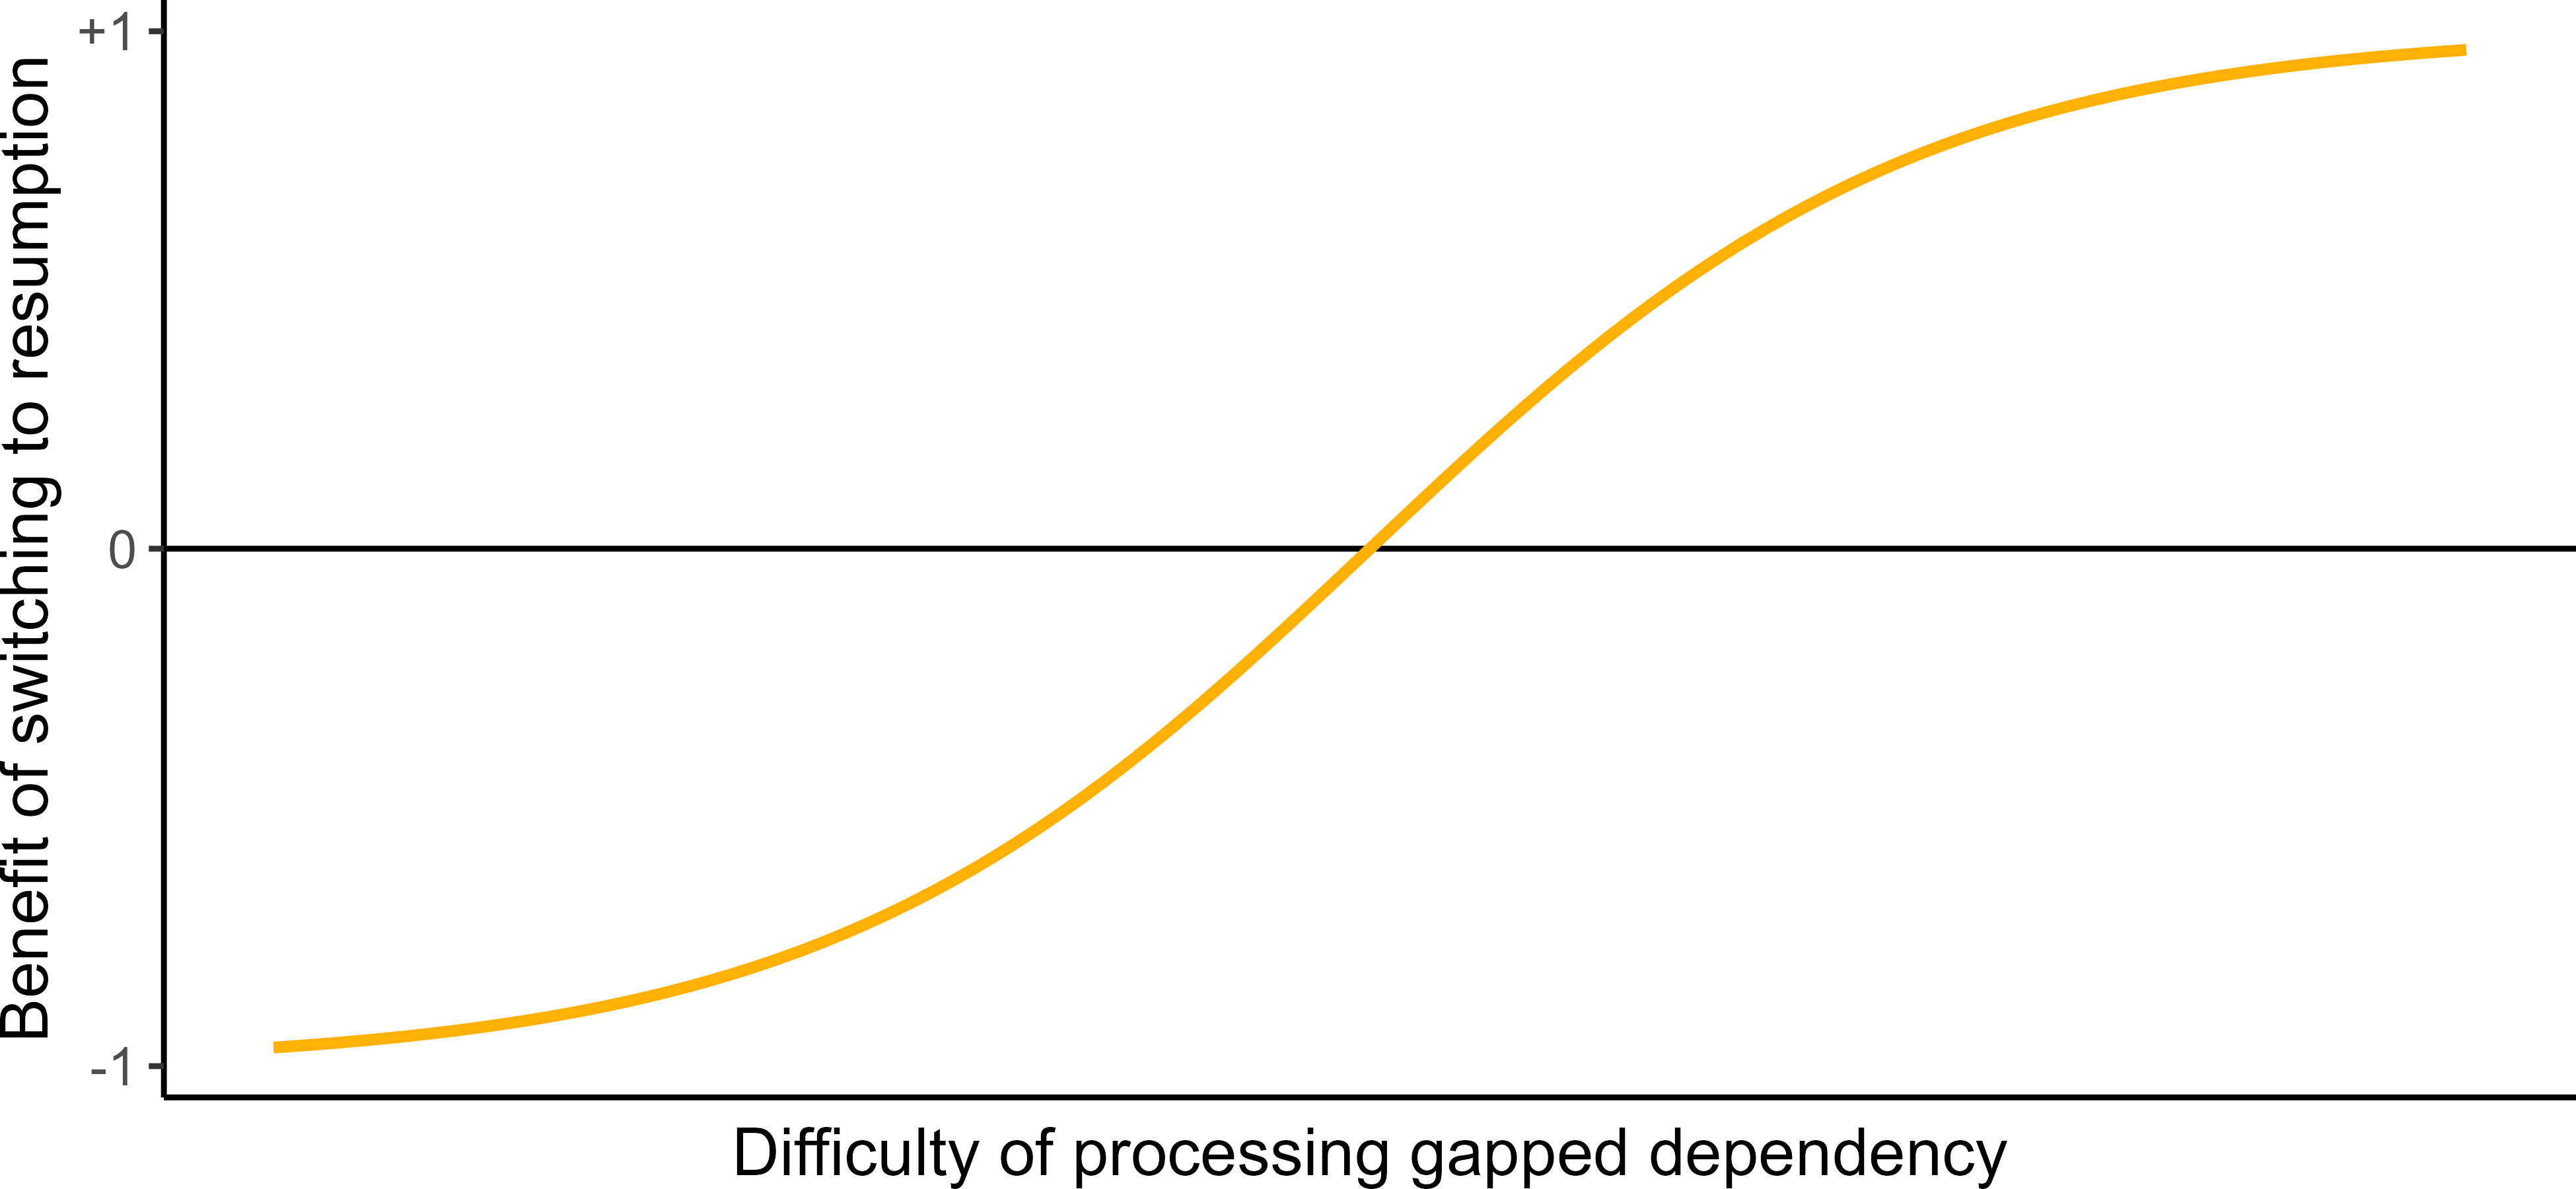
\includegraphics{../analysis/plots/sigmoid.png}
\vspace{-12pt}
\end{figure}

\noindent The processor tends to favor gapping over resumption at the lower end of the difficulty spectrum, such as in short-distance SRCs, and it tends to favor resumption over gapping at the upper end of the spectrum, such as in long-distance RCs that extend into islands.

If gapping tends to be preferred in easy-to-process RCs and resumption tends to be preferred in difficult-to-process RCs, then we can look upon the gapping vs. resumption opposition as just one more example of the push and pull between competing pressures (economy vs. explicitness, etc.) that is so characteristic of human language processing in general (\cite{hawkins2004}, p.~13ff; \cite{hawkins2014}, p.~201ff; \cite{casasanto.sag2008}, p.~605).

%========================================================%
\section{Summing up}\label{res-conclusion}
%========================================================%

In this chapter, we have reviewed the L1 experimental literature on the acceptability and real-time processing of gapped vs. resumptive RCs. On the acceptability front, we have seen that linguists today tend to regard resumption in English as an ungrammatical repair strategy. On the processing front, we have seen that while it is widely acknowledged that resumption facilitates RC production---both in intrusive resumption languages like English and in grammatical resumption languages like Hebrew---opinions differ on the matter of whether resumption can also facilitate RC comprehension. Supporters of the selfish speaker model argue that resumption hinders RC comprehension. By contrast, an opposing point of view holds that gapping and resumption in RCs both come with advantages and disadvantages that cause gapping to be facilitatory in some contexts and resumption to be facilitatory in others. One of the main goals of the present dissertation is to put these conflicting ideas to the test, drawing on psycholinguistic methods that have been utilized in this area of research in recent years and making changes where needed to correct for shortcomings in previous studies. Whereas the primary focus in this chapter has been on L1 adults, in the next chapter we turn to the literature on RC resumption among L2ers.